\documentclass[a4paper]{article}
%\usepackage[T1]{fontenc}
\usepackage[english]{babel}

\usepackage{amsmath}
\usepackage{amssymb,amsfonts,textcomp, graphicx}
\usepackage{graphics}

\usepackage{wrapfig}

\usepackage{parskip}

\usepackage{color}
\usepackage{array}
\usepackage{hhline}
\usepackage{subcaption}

\usepackage{textcomp}

\usepackage[hidelinks]{hyperref}

\setlength\tabcolsep{1mm}
\renewcommand\arraystretch{1.3}

\setlength\voffset{-1in}
\setlength\hoffset{-1in}
\setlength\topmargin{0.7874in}
\setlength\oddsidemargin{0.7874in}
\setlength\textheight{10.118099in}
\setlength\textwidth{6.6932993in}
\setlength\footskip{0.0cm}
\setlength\headheight{0cm}
\setlength\headsep{0cm}


\begin{document}

\newcommand\textstyleEmphasis[1]{\textit{#1}}
\renewcommand{\contentsname}{Table des mati\`eres}
\renewcommand\refname{R\'ef\'erences}

\renewcommand{\abstractname}{Pr\'eambule}
\title{\textbf{Projet Circuits Int\'egr\'es Radiofr\'equence \\ Conception d'un LNA \`a 2.45 GHz \\ en Technologie 0.35 $\mu$m AMS}}
\author{Mohamed Hage Hassan \\ Cl\'ement Cheung}
\date{12 D\'ecembre 2017}
\maketitle
\thispagestyle{empty}

\tableofcontents
\clearpage

\iffalse

\begin{figure}[!htb]
\begin{center}
  \includegraphics[scale=0.47]{Echantillonneur-bloqueur.png}
  \caption{Sch\'ema d'un \'echantilloneur-bloqueur \`a capacit\'e commut\'ee}
\end{center}
\end{figure}

\begin{figure}[!htb]
  \begin{subfigure}[t]{.5\linewidth}
      \centering
      \includegraphics[width=1.1\linewidth]{circuit-RC.png}
      \label{fig:rccircuit}
  \end{subfigure}%
  \begin{subfigure}[t]{.5\linewidth}
    \centering
    \includegraphics[width=1.1\linewidth]{sim-inital.png}
    \label{fig:rccircuit-sim}
  \end{subfigure}%
  \caption{Sch\'ema et Simulation du circuit}
  \label{fig:RC-sim}
\end{figure}

\fi

\section*{Introduction}
\addcontentsline{toc}{section}{Introduction}

\vskip 7 cm

\section{Conception du LNA - Partie th\'eorique}
On essaye de concevoir l'amplificateur faible bruit (figure. \ref{lna-ams})

\begin{figure}[!htb]
\begin{center}
  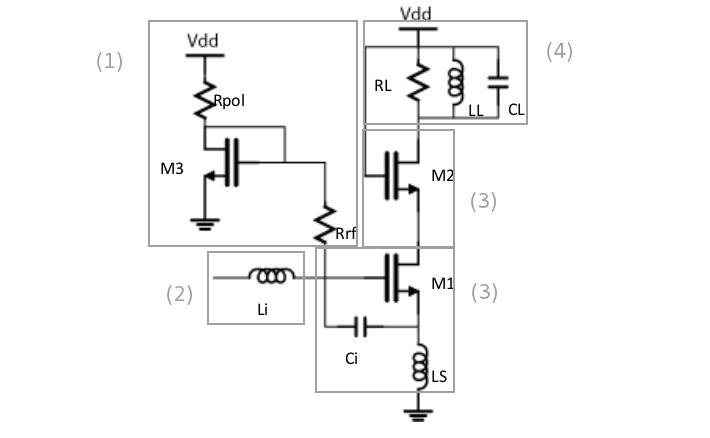
\includegraphics[scale=0.47]{lna-anotated.png}
  \caption{Sch\'ema de l'amplificateur faible bruit\cite{RFIC-tp-lna}}
  \label{lna-ams}
\end{center}
\end{figure}

Le sch\'ema comporte : \textbf{\textcolor{red}{Explication ::}}
\begin{enumerate} \itemsep -3pt
  \item Circuit de polarization
  \item Inductance de shock $L_i$
  \item \'Etage cascode avec l'adaptation
  \item Circuit r\'esonant parall\`ele RLC
\end{enumerate}

Le LNA doit respecter un cahier de charge bien d\'efini :
\begin{itemize} \itemsep -3pt
  \item $Gv = 20 (26 db)$, $F = 1.5 (1.76 db)$, $IIP3 = -10 dbm$
  \item $F_0 = 2.45 GHz$
  \item$\gamma = 0.82$
  \item $C_{ox} = 5 \times 10^{-3} pF/\mu m^2 $, $k_n = 80 \mu A/V^2$
  \item Courant de polarization : $I_{DS0} = 1.5 mA$
  \item Capacit\'e en sortie $C_L = 1 pF $
  \item $Q_e = 2$
\end{itemize}


\subsection{Calcul de la charge}
On cherche $L_L$ pour r\'esoner \`a $2.45 GHz$ : Pour un circuit RLC parall\`ele,
la fr\'equence de r\'esonance est donn\'ee par :
\[
  \omega_0 = \frac{1}{\sqrt{L_L C_L}} \implies L_L = \frac{1}{(2\pi F_0)^2 C_L}
\]
Pour $F_0 = 2.45 GHz$ et $C_L = 1 pF$, on a $L_L = 4.21 nH$.

\textbf{Calcul de $g_m$:}\\
Connaissant $L_L$ et le facteur de bruit F, on cherche \`a retrouver la transductance $g_m$ :
\[
  F = 1 + \frac{\gamma}{50 gm} \frac{1}{Q^2_e}
\]
\[
  \implies gm = \frac{\gamma}{50 (F-1) Q^2_e}
\]
Ce qui nous donne $g_m = 8.2 \times 10^{-3} \Omega^{-1}$, pour $Q_e = 2$, $F = 1.5$ et $\gamma = 0.82$.

\textbf{Calcul de $R_L$:}\\
Pour $G_v = 20$, $g_m = 8.2 \times 10^{-3} \Omega^{-1}$, et $Q_e = 2$, on a :
  \[
    G_v = g_m R_L Q_e \implies R_L = \frac{G_v}{g_m Q_e} = 1.219 k\Omega
  \]

\subsection{Dimensionnement du transistor et calcul du r\'eseau d'entr\'ee}
\textbf{Capacit\'e totale $C_i$ // $C_{gs}$:}\\
Le coefficient de qualit\'e $Q_e$ pour un circuit RC s\'erie :
\[
  Q_e = \frac{||X||}{R} \phantom{4}\phantom{4}\phantom{4} X = \frac{1}{\omega_0 C_{tot}}
\]
\[
\implies C_{tot} = \frac{1}{\omega_0 Q_e 50} = 0.64 pF
\]
\textbf{Pour la partie suivante, on ne consid\`ere que le transistor $M_1$}:\\
La transductance $g_m$ d'un MOSFET s\'exprime par :
\[
  g_m = 2\sqrt{K_n \bigg( \frac{W}{L} \bigg)_{(M_1)} I_{DS0}}
\]
\[
\implies \bigg(\frac{W}{L}\bigg)_{(M_1)}  = \frac{g^2_m}{4 k_n I_{DS0}} = 140.08
\]
Pour la technologie AMS 0.35 $\mu$m, o\`u $L = L_{min} = 0.35 \mu m$, on retrouve $W = 49.02 \mu m$.\\
Connaissant W, c'est possible de calculer la capacit\'e parasite $C_{gs}$ entre la source et le gate.
\[
C_{gs} = \frac{1}{2} C_{ox} W L = 42.89 fF
\]

\textbf{Calcul de $C_i$, $L_S$ :}\\
Sachant que $C_{tot}$ de l'entr\'ee est form\'ee par $C_i$ et la capacit\'e parasite $C_{gs}$, on a :
\[
  C_i = C_{tot} - C_{gs} = 0.64\times 10^{-12} - 42.89 \times 10^{-15} = 0.597 \times 10^{-12} pF
\]
En se basant sur \cite{RFIC-cours}, on sait que l'\'element $L_S$ du circuit d'adaptation en entr\'ee
doit \^etre adapt\'e \`a $50 \Omega$ :
\[
  L_S \omega_T = 50 \implies L_S = \frac{50}{\omega_T} = \frac{50}{(g_m)_{M_1}}C_{gs} = 0.26 nH
\]

\clearpage
\textbf{Calcul de la tension de d\'epassage $V_{OD}$, $L_i$:}
La transductance du MOSFET poss\`ede plusieurs expressions :
\[
  g_m = 2\sqrt{K_n \bigg( \frac{W}{L} \bigg)_{(M_1)} I_{DS0}} = \frac{2 I_{DS0}}{V_{gs} - V_{t}}
\]
On peut remonter \`a la tension de d\'epassage : $V_{OD} = V_{gs} - V_/{t}$:
\[
  V_{gs} - V_{t} = \frac{2 I_{DS0}}{g_m} = 0.36 V
\]
Pour $L_i$, on a
\[
  \omega_0 = \frac{1}{\sqrt{(L_g + L_s) C_{gs}}} \implies L_g + L_S = \frac{1}{\omega^2_0 C_{gs}}
\]
Ce qui nous donne :
\[
  L_i = L_g = \frac{1}{\omega^2_0 C_{gs}} - L_{S} = 98.2 nH
\]

\section{Partie pratique}
\subsection{Simulation DC du transistor seul}

\subsection{Adaptation de la partie r\'eelle de l'imp\'edance d'entr\'ee}

\subsection{Polarisation}
\subsection{Gain}
\subsection{Adaptation de la partie imaginaire de l'imp\'edance d'entr\'ee du LNA}
\subsection{Facteur de bruit}

\clearpage
\section*{Conclusion}
\addcontentsline{toc}{section}{Conclusion}




\addcontentsline{toc}{section}{R\'ef\'erences}
\begin{thebibliography}{9}

\bibitem{RFIC-tp-lna}
\textit{Conception d'un LNA \`a 2.45 GHz en Technologie 0.35 $\mu$m AMS - \'Enonc\'e de TP}\\
\texttt{Institut Polytechnique de Grenoble - Phelma}

\bibitem{RFIC-cours}
\textit{Radio Frequency Integrated Circuits Course}\\
\texttt{Sylvain Bourdel, Florence Podevin, Institut Polytechnique de Grenoble - Phelma}

\bibitem{conception-adaptation}
\textit{Conception d'un circuit en L \`a l'aide de l'abaque de Smith}\\
\texttt{http://f5zv.pagesperso-orange.fr/RADIO/RM/RM23/RM23p/RM23p03.html}

\bibitem{Analog-CMOS-microelectronics}
\textit{Design of Analog CMOS Integrated Circuits, 2nd Edition}\\
\texttt{Behzad Razavi, McGraw-Hill Education}

\bibitem{conception-circuits-integrees}
\textit{Conception de circuits int\'egr\'es analogique}\\
\texttt{Laurent Aubard, Institut Polytechnique de Grenoble - Phelma}

\end{thebibliography}


\end{document}
